\chapter{\label{chap:modeling}Modelagem do Sistema}

Conforme visto na subseção \ref{subsec:simulation:components}, um sistema de
simulação possui uma série de componentes conceituais, cada um com suas
responsabilidades bem definidas. Para projetar um simulador, diversas abordagens
e paradigmas poderiam ser aplicadas. Para o projeto do simulador de sistemas de
elevadores deste estudo, doravante chamado apenas de simulador, optou-se pelo
paradigma de \textit{Programação Orientada a Objetos}. Esta escolha se deu pelos
seguintes motivos:

\begin{description}
  \item[Capacidade de Abstração]\hfill \\
    Conceitos da Programação Orientada a Objetos, como classes, interfaces,
    polimorfismo, herança e sobrecarga permitem a realização de uma modelagem
    conceitual em alto nível de abstração, permitindo uma explanação de fácil
    entendimento sem ser necessário abordar questões da implementação em si
    (linguagem de programação, arquitetura, etc).
  \item[Padrão de Mercado]\hfill \\
    Desde meados dos anos 90, a Programação Orientada a Objetos tornou-se
    frequentemente utilizada no mercado de desenvolvimento de software e nos
    ambientes acadêmicos relacionados à computação. Assim, é possível atingir
    uma maior audiência.
  \item[Domínio dos Autores]\hfill \\
    O paradigma é de domínio dos autores deste estudo.
\end{description}

Nas próximas seções serão apresentadas as modelagens conceituais para o projeto
do simulador de elevadores.

\section{\label{sec:eventos-e-tipos}Eventos e tipos}

A simulação de eventos discretos, como o próprio nome já diz, é orientada a
eventos. Isso significa dizer que as alterações no estado do sistema ocorrerão
somente na ocasião de algum evento e é preciso ser possível representar um
evento no contexto do simulador.

Um evento é uma estrutura que deve possuir as seguintes informações: (1) o tipo
do evento; (2) o horário agendado para a ocorrência do evento; (3) um cliente
(passageiro) e/ou (4) um elevador e/ou (5) um andar do prédio. As existência de
informações para os itens (3), (4) e (5) dependem do tipo de evento, que pode
ser uma das seguintes opções:

\newpage

\begin{description}
  \item[Chegada de grupo de clientes] \hfill \ um grupo de clientes chegou na fila de um andar.
  \item[Chegada de elevador] \hfill \ um elevador chegou a um andar e abriu as portas.
\end{description}

Para o evento \textbf{chegada de um cliente}, é necessário conhecer o cliente e
o andar. Para o evento \textbf{chegada de um elevator}, é necessário conhecer o
elevador e o andar. A figura \ref{fig:diagram:event} exibe o diagrama de classes
para eventos (classe \textit{Event}) e tipos de evento (enumeração
\textit{EventType}). Adicionalmente foi criada a classe \textit{Config},
responsável por armazenar informações referentes ao cenário sendo simulado.

\begin{figure}[htb!]
  \centering
  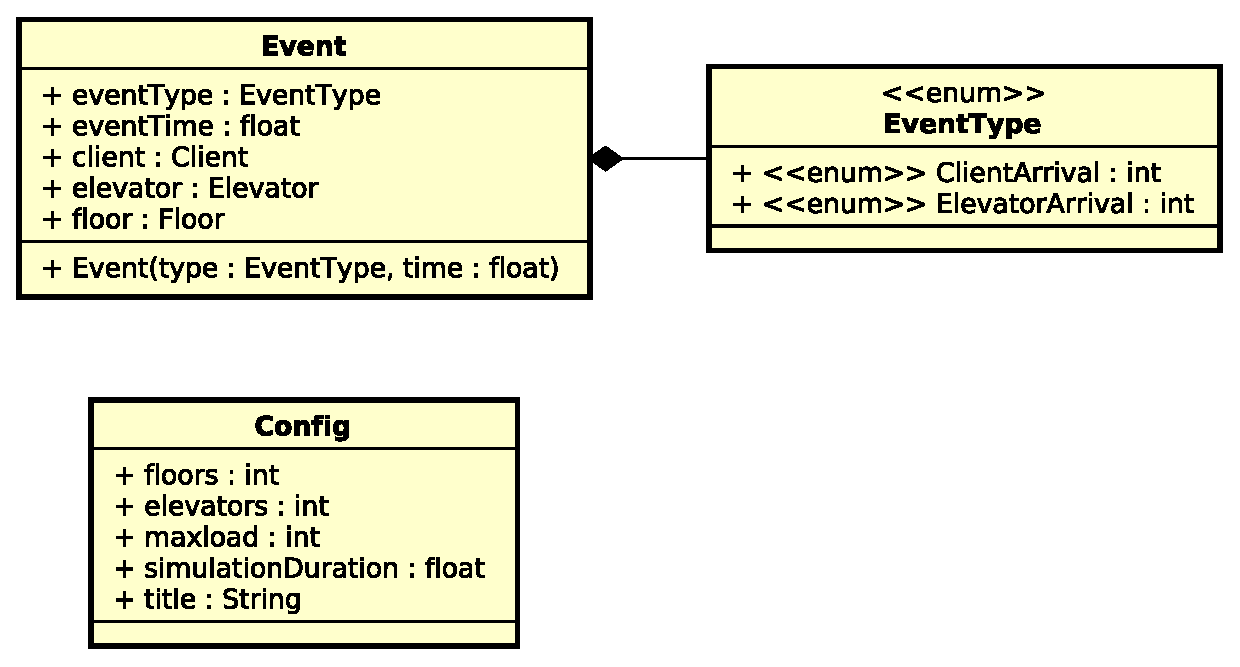
\includegraphics[scale=0.6]{img/Basic.eps}
  \caption[Diagrama de classes para eventos, tipos e configuração]{Diagrama de classes para eventos, tipos de eventos e configuração da simulação.}
\label{fig:diagram:event}
\end{figure}

\section{\label{sec:reactive}Componentes reativos}

Durante a execução da simulação, à medida que eventos ocorrem, componentes do
simulador deverão alterar seu estado interno de acordo com o evento ocorrido,
levando o estado do simulador a uma nova situação. Estes componentes são:

\begin{enumerate}
  \item Relógio da Simulação;
  \item Estado do Sistema;
  \item Contadores Estatísticos.
\end{enumerate}

A seguir são apresentadas as classes que representam estes componentes no
simulador.

\subsection{Estado do sistema}

Entre os componentes fundamentais de um simulador destaca-se a representação do
\textit{estado do sistema}, uma coleção de variáveis necessárias para descrever
o sistema em um instante em particular da simulação \cite{Law}. Neste projeto, a
classe \textit{Building} é responsável por encapsular o conjunto de informações
que definem este estado (figura \ref{fig:diagram:model}). Esta classe é
responsável por gerenciar múltiplas instâncias de elevadores (classe
\textit{Elevator}), andares (classe \textit{Floor}) e clientes (classe
\textit{Client}) e relacionar estas instâncias entre si - reproduzindo, deste
modo, as dinâmicas do sistema do mundo real que está sendo simulado.

\begin{figure}[htb!]
  \centering
  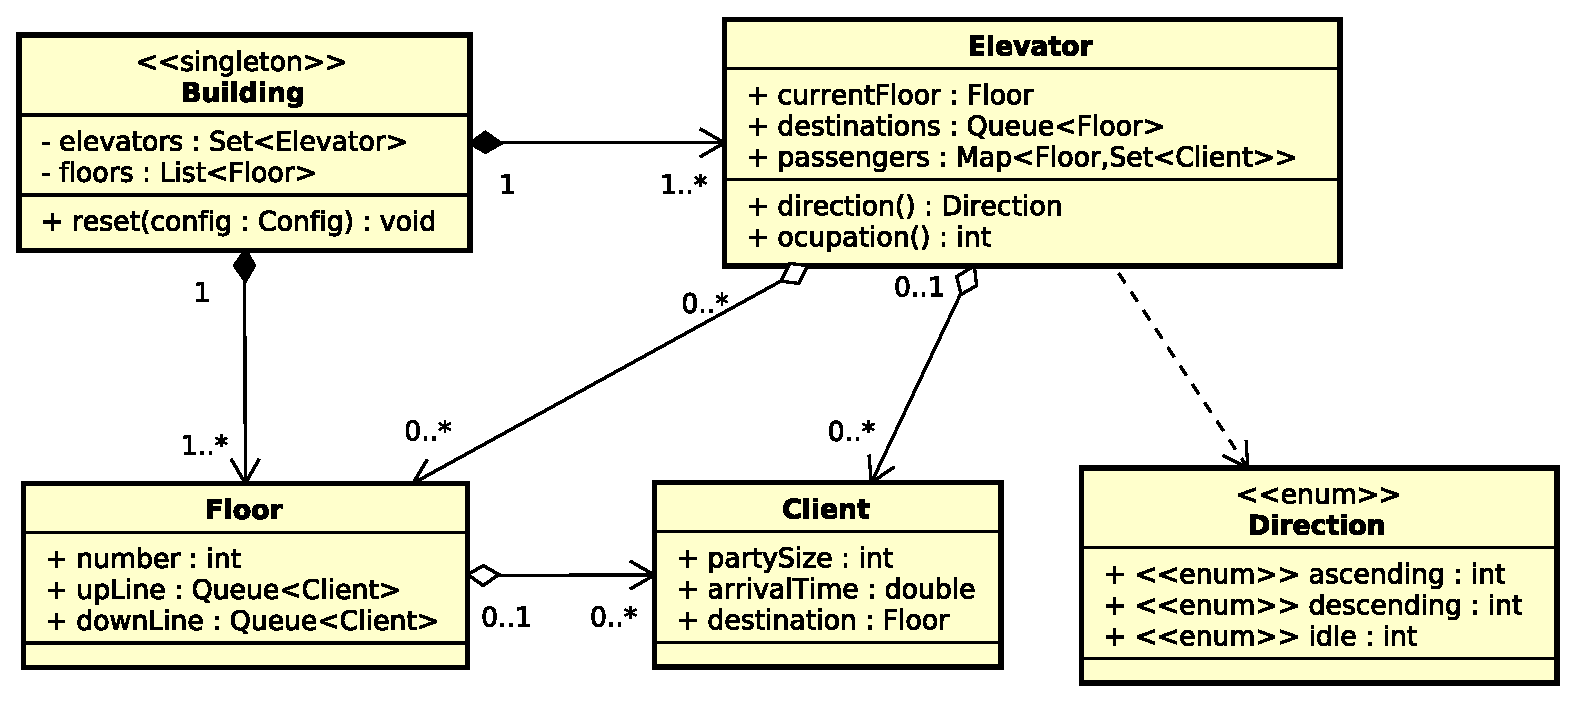
\includegraphics[scale=0.6]{img/Model.eps}
  \caption{Diagrama de classes do \textit{Estado do Sistema}.}
\label{fig:diagram:model}
\end{figure}

\begin{description}
  \item[Building] \hfill \\
    Representa a composição do prédio sendo simulado. Possui um conjunto de
    elevadores, uma lista ordenada de andares e um método \texttt{reset},
    utilizado para a inicialização da simulação. Um prédio é formado por no
    mínimo um elevador e no mínimo um andar\footnote{Isto em termos conceituais;
    porém, não há sentido na existência de um sistema de elevadores em uma
    edificação com somente um andar. De fato, conforme afirmado na seção
    \ref{section:scenarios}, serão simulados prédios com, no mínimo, 4
    andares.}.

  \item[Floor] \hfill \\
    Parte componente de um prédio, possuindo uma numeração e duas
    filas\footnote{No mundo real, apesar de aparentemente as pessoas formarem
    uma fila única, os membros da fila respeitam o sentido de viagem do elevador
    e implicitamente separam-se em duas filas: uma para subir e outra para
    descer.}: uma para clientes que desejam descer e outra para clientes que
    desejam subir.

\item[Elevator] \hfill \\
    Representa um elevador. Possui como atributos o andar em que se
    encontra, uma sequência ordenada de andares de destino e um mapa associando
    andares com conjuntos de clientes - ou seja, para cada andar o mapa reune
    quais os grupos de clientes que o possuem como destino. Além disso, possui
    métodos auxiliares para informar o sentido da viagem do elevador
    (\texttt{direction}), bem como a sua ocupação atual (\texttt{occupation}).

\item[Client] \hfill \\
    Representa um grupo de pessoas que desejam utilizar um elevador. Possui como
    atributos o número de pessoas no grupo (\texttt{partySize}), o horário em
    que chegou na fila do andar (\texttt{arrivalTime}) e o andar destino para o
    qual deseja ir (\texttt{destination}).

\end{description}

\subsection{Relógio da simulação}

O \textit{relógio da simulação} é representado pela classe \textit{Timer}
(figura \ref{fig:diagram:timer}). Esta classe encapsula o acesso ao atributo
privado \texttt{time}, provendo métodos para inicialização (\texttt{reset}),
consulta (\texttt{currentTime}), atualização para um valor arbitrário
(\texttt{advanceTo}) e atualização por incremento (\texttt{advanceBy}).

\begin{figure}[htb!]
  \centering
  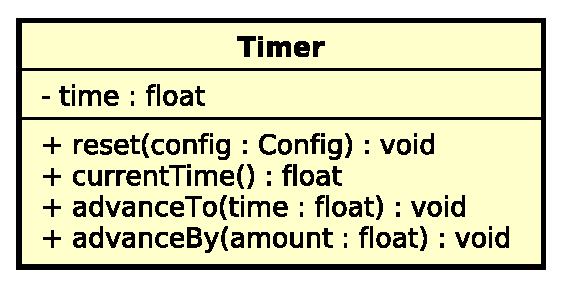
\includegraphics[scale=0.6]{img/Timer.eps}
  \caption{Diagrama de classes do \textit{Relógio da Simulação}.}
\label{fig:diagram:timer}
\end{figure}

\subsection{Contadores Estatísticos}

Os \textit{contadores estatísticos} da simulação são responsáveis por coletar e
sumarizar dados do sistema durante toda a execução da simulação. Sua existência
permite a realização de análises qualitativas e quantitativas a respeito do
sistema simulado.

Neste projeto, os \textit{contadores estatísticos} são representados pela classe
\textit{Statistics} (figura \ref{fig:diagram:stats}). Conforme descrito na
proposta de trabalho deste estudo, o objetivo é encontrar algoritmos que
otimizem o tempo de espera médio. Porém, armazenar mais dados estatísticos
permite realizar análises mais ricas, fornecendo informações como desvios, por
exemplo. Portanto, para cada grupo de clientes transportados pelo sistema serão
armazenados o seguinte conjunto de informações sobre a viagem (classe
\textit{Travel}):

\newpage

\begin{description}
  \item[\texttt{origin}] \hfill \\ O andar de origem da viagem.

  \item[\texttt{client}] \hfill \\
    O grupo de cliente, contendo o tamanho do grupo, a hora em que
    chegou à fila e o seu andar de destino.

  \item[\texttt{elevator}] \hfill \\
    O elevador que transportou o grupo do andar origem ao andar destino.

  \item[\texttt{waitingTime}] \hfill \\
    O tempo que o grupo esperou na fila - ou seja, o tempo compreendido entre a
  chegada do grupo na fila e o seu embarque no elevador.

  \item[\texttt{journeyTime}] \hfill \\
    O tempo que o grupo esperou na fila - ou seja, o tempo compreendido entre
    o embarque do grupo no elevador e o desembarque no andar destino.

  \item[\texttt{arrivalTime}] \hfill \\
    O horário em que o grupo desembarou no andar destino.
\end{description}

Além destes, a classe também possui métodos para inicialização (\texttt{reset})
e para avaliar se a simulação deve terminar (\texttt{keepRunning})~-~por
exemplo, o tempo mínimo se simulação já se passou.

\begin{figure}[htb!]
  \centering
  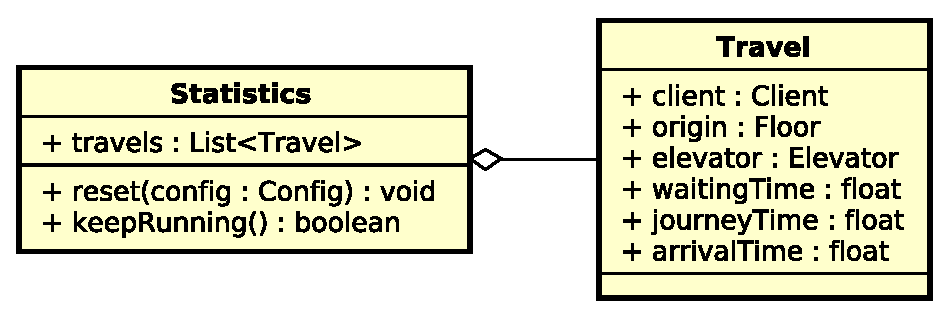
\includegraphics[scale=0.6]{img/Stats.eps}
  \caption{Diagrama de classes do \textit{Contadores Estatísticos}.}
\label{fig:diagram:stats}
\end{figure}

\section{\label{sec:model:event}Gerenciamento de eventos}

Na seção \ref{sec:reactive} foram apresentados componentes reativos~-~ou seja,
que devem reagir na ocorrência de um evento. Porém restam as questões de como
saber qual evento será o próximo a ocorrer e como notificar os elementos
reativos disso. Portanto, precisamos de mecanismos para ordenar eventos e
notificar os componentes da ocorrência de um evento.

\subsection{Organização e priorização}

Na seção \ref{chap:sim:timeadvance} foi apresentado o \textit{mecanismo de
avanço de tempo para o próximo evento}, onde deve-se verificar, em uma lista de
eventos, qual é o próximo evento a ocorrer. Dado um conjunto de eventos
agendados (ou seja, ainda não ocorridos), o primeiro evento a ocorrer é
justamente o que possui o menor tempo de agendamento. Um tipo abstrato de dados
que serve para este propósito é uma \textit{fila prioritária}, ou
\textit{priority queue}, que funciona de forma similar a filas \textit{FIFO},
com a diferença de que cada elemento armazenado possui uma prioridade associada.
A \textit{fila prioritária} irá atender os elementos por ordem de prioridade, da
maior para a menor. Ao considerar que a prioridade de um evento é inversamente
proporcional ao instante em que irá ocorrer - ou seja, quanto menor o tempo do
evento maior é a sua prioridade -, temos uma fila na qual o próximo elemento a
ser atendido sempre será o próximo evento a ocorrer.

Assim, a classe \textit{EventQueue} encapsula uma fila prioritária de eventos,
fornecendo métodos para inserir um evento na fila (\texttt{push}), recuperar e
remover o próximo evento (\texttt{pop}) ou simplesmente ``espiar'' o próximo
evento (\texttt{peek}). Juntamente com a classe
\textit{EventGenerator}\footnote{Classe responsável pela criação de eventos;
abordada mais adiante neste estudo.}, a \textit{EventQueue} compõe o chamado
\textit{Sistema de Priorização de Eventos}, ou \textit{SPE}. Assim,
possibilita-se que facilmente se saiba qual será o próximo evento a ocorrer.

\begin{figure}[htb!]
  \centering
  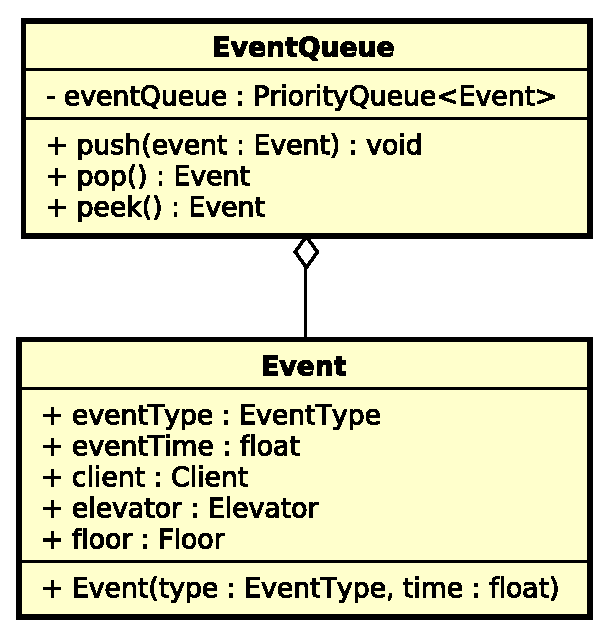
\includegraphics[scale=0.6]{img/EventQueue.eps}
  \caption{Diagrama de classes do \textit{Sistema de Priorização de Eventos}.}
\label{fig:diagram:event:manage}
\end{figure}

\subsection{\label{sec:model:notify}Notificação}

Quando o próximo evento a ocorrer é conhecido, o problema passa a ser notificar
os elementos reativos que este evento ocorreu para que os mesmos possam
atualizar seus estados internos. De acordo com Gamma
\cite{Gamma:1995:DPE:186897}, o padrão \textit{Observer} é um \textit{design
pattern} indicado para resolver este problema. Este \textit{pattern} define uma
dependência de um-para-muitos ($1:N$) entre objetos de modo que, quando este um
objeto (\textit{subject}) tem seu estado alterado, todos os seus dependentes
(\textit{observers}) são notificados deste mudança. Por consequência, estes
dependentes podem modificar seu estado interno baseando-se nas informações desta
notificação. Neste projeto, o subsistema que segue o \textit{Observer pattern}
será chamado de \textit{Sistema de Notificação de Eventos}, ou \textit{SNE}.

Os três principais componentes do \textit{SNE} (figura
\ref{fig:diagram:notification}) são duas interfaces e uma classe:

\begin{description}
  \item[EventObserver] \hfill \\
    Interface a ser realizada por qualquer classe que deseje receber
    notificações de eventos. Seu único método, \texttt{notify}, permite o
    recebimento de uma notificação de um evento.

  \item[EventNotifier] \hfill \\
    Interface a ser realizada por qualquer classe que deseje notificar a
    ocorrência de eventos. Define métodos que objetos que implementem a
    interface \textit{EventObserver} possam registrar (\texttt{register}) ou
    desregistrar (\texttt{unregister}) para receber notificações de ocorrências
    de um determinado tipo de evento, além do método \texttt{notify}, que deverá
    notificar um evento para todos os \textit{observers} registrados.

\item[EventDispatcher] \hfill \\
    Classe concreta que realiza a interface \textit{EventNotifier}. Deve possuir
    uma estrutura de dados para armazenar quais \textit{observers} se
    registraram para cada tipo de evento. Na ocorrência de um evento, o
    \textit{EventDispatcher} é responsável por varrer a lista de
    \textit{observers} registrados e notificá-los de acordo com o tipo de evento
    ocorrido.

\end{description}

\begin{figure}[htb!]
  \centering
  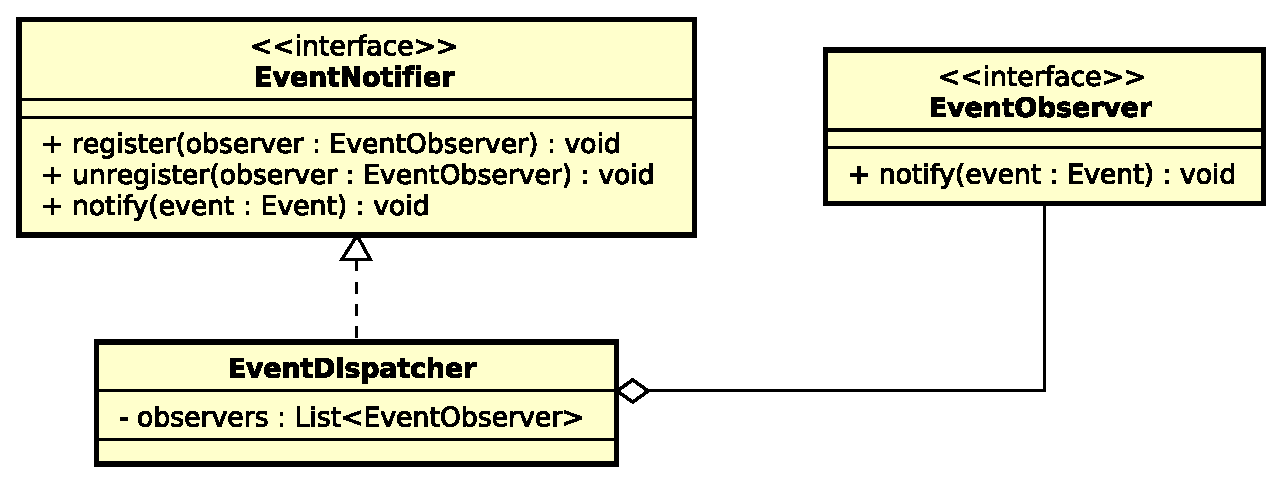
\includegraphics[scale=0.6]{img/Notification.eps}
  \caption{Diagrama de classes do \textit{Sistema de Notificação de Eventos}.}
\label{fig:diagram:notification}
\end{figure}

Três importantes componentes do simulador podem se beneficiar desta construção:
(1) o \textit{relógio do sistema} (classe \textit{Timer}); (2) os
\textit{contadores estatísticos} (classe \textit{Statistics}); e (3) o
\textit{estado do sistema} (classe \textit{Building}). Na ocorrência de um
evento, estas três entidades devem ser notificadas e cada uma irá alterar seu
estado interno da forma adequada. Para isto, devem implementar a interface
\textit{EventObserver} e registrarem-se no \textit{EventDispatcher}, conforme
ilustrado na figura \ref{fig:diagram:observers}. Assim, o
\textit{EventDispatcher} e a \textit{EventQueue} podem, juntos, notificar aos
componentes reativos exatamente qual evento ocorreu em cada iteração da
simulação, na ordem correta dos eventos.

\begin{figure}[htb!]
  \centering
  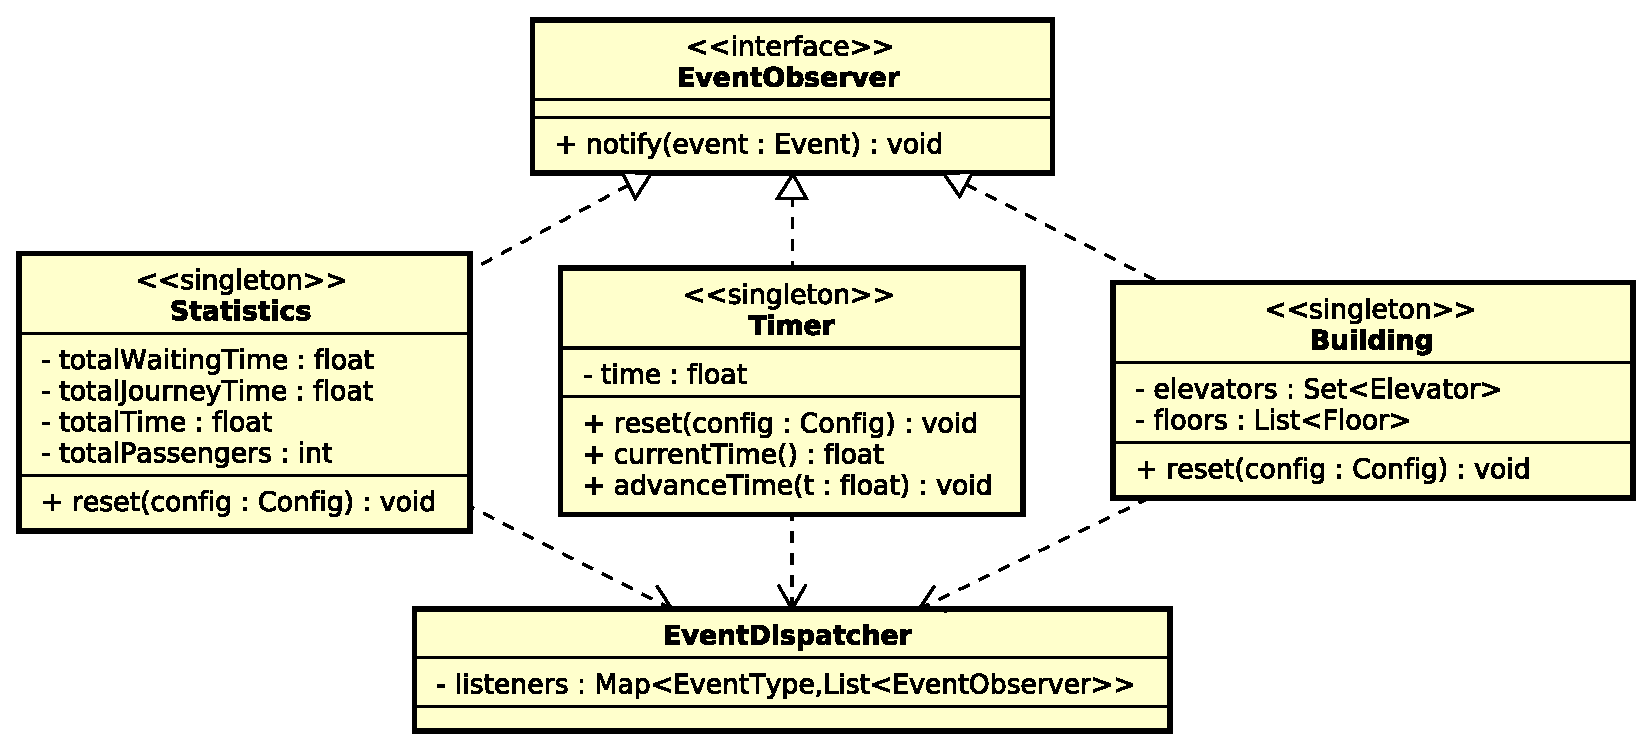
\includegraphics[scale=0.6]{img/Observers.eps}
  \caption{Diagrama de classes dos \textit{observers}.}
\label{fig:diagram:observers}
\end{figure}

\section{\label{sec:model:generator}Criação}

Como foi mostrado na Seção~\ref{sec:eventos-e-tipos}, há dois eventos possíveis:
\textbf{chegada de passageiros} e \textbf{chegada de elevador a um andar}.

A chegada de um elevador é um evento determinístico~-~sabe-se que o elevador
viaja a uma velocidade constante e conhece-se sua agenda interna. Portanto o
tempo entre um elevador sair de um andar e o evento deste chegar a outro andar é
fixo. Isto é, para um elevador que leva $t$ segundos para se deslocar um andar,
após sair de um andar $a_{0}$ no tempo $t_{0}$ e subir ou descer $a$ andares, o evento
de chegar ao andar $a_{0} + a$ ocorrerá no tempo $t_{0} + at$.

Já a chegada de passageiros segue modelos estocásticos, descritos na Seção~\ref{chap:input}.

A Figura~\ref{fig:diagram:generator} mostra o diagrama UML da classe que gera eventos.

\begin{figure}[htb!]
  \centering
  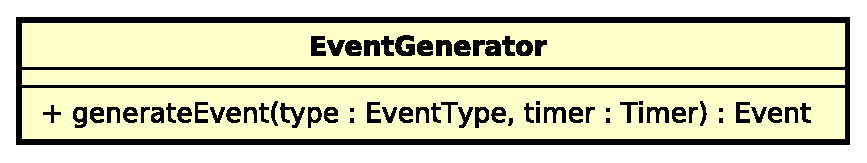
\includegraphics[scale=0.6]{img/EventGenerator.eps}
  \caption{Diagrama de classes do \textit{Sistema de Geração de Eventos}.}
\label{fig:diagram:generator}
\end{figure}

\subsection{\label{chap:input}Entrada de Distribuição de Probabilidade}

\textbf{TO-DO! TO-DO! TO-DO! TO-DO! TO-DO!}

\textbf{TO-DO! TO-DO! TO-DO! TO-DO! TO-DO!}

\textbf{TO-DO! TO-DO! TO-DO! TO-DO! TO-DO!}

\textbf{TO-DO! TO-DO! TO-DO! TO-DO! TO-DO!}

Segundo~\cite{Ross:2006:IPM:1197141}, bla bla bla whiskas sachê.

Aqui vamos apresentar:

\begin{itemize}
\item Conceitos sobre distribuições de probabilidade;
\item Conceitos sobre geração de variáveis aleatórias em ambiente computacional;
\item Descrever o modelo selecionado de processo de chegada de clientes
(passageiros);
\item Algoritmos e fluxogramas dos eventos do simulador que causarão alterações
no estado do sistema.
\end{itemize}

\section{\label{sec:model:report}Geração de relatórios}

Por último mas não menos importante, é apresentada a classe
\textit{ReportBuilder}, ilustrado pela figura \ref{fig:diagram:report}. Esta
classe tem por responsabilidade a elaboração de um relatório (em arquivo) a
partir da configuração da simulação e das estatísticas acumuladas durante a
execução.

\begin{figure}[htb!]
  \centering
  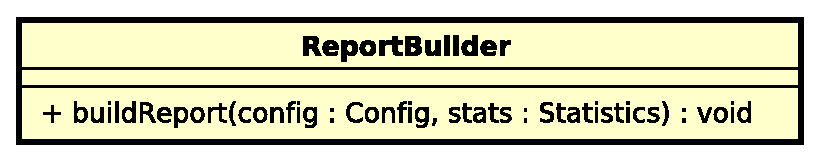
\includegraphics[scale=0.6]{img/Report.eps}
  \caption{Diagrama de classes do \textit{ReportBuilder}.}
\label{fig:diagram:report}
\end{figure}

\newpage

\subsection{Exemplo de Relatório}

\begin{lstlisting}
Título:       Prédio comercial de tamanho médio
Andares:      99
Elevadores:   99
Carga máxima: 99
Algoritmo:    Planning (horizonte 9)
---------------------------------------------------
Período simulado: 99 horas
Horário inicial:  00:00:00
Horário final:    23:59:59
---------------------------------------------------
Passageiros transportados: 99
Total de paradas: 999

       Total    Média   Desvio
AWT    99999    99999    99999
AJT    99999    99999    99999
---------------------------------------------------
Simulação executada em 99:99:99.
\end{lstlisting}

\section{Simulador completo}

O uso de instâncias de todas estas classes juntas dá forma ao simulador,
conforme proposto por \cite{Law,Banks}. Entretanto, todas as interações entre as
instâncias devem ser organizadas conforme o fluxo proposto na figura
\ref{fig:simflow}. O componente responsável por orquestrar estas interações e
garantir o fluxo de execução é representado pela classe \textit{Simulator}.

Esta classe não possui atributos ou métodos específicos; somente as instâncias
das outras classes e um método que realiza um laço indefinido, onde um evento é
recuperado e notificado para os componentes reativos; estes, por sua vez,
atualizam seu estado interno e agendam novos eventos; a simulação segue até que
a condição de parada seja satisfeita. O algoritmo \ref{alg:sim} mostra um
pseudo-código de como poderia ser este método de execução da simulação.

\begin{figure}[htb!]
  \centering
  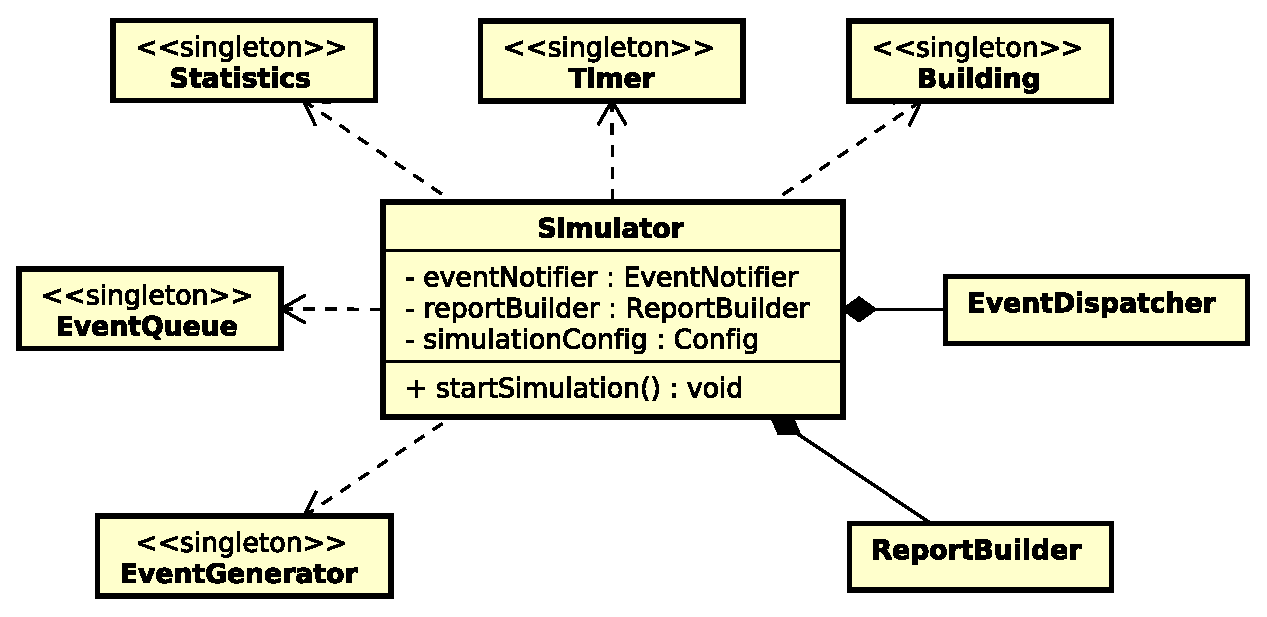
\includegraphics[scale=0.6]{img/Simulator.eps}
  \caption{Diagrama de Classes do Simulador}
\label{fig:diagram:simulator}
\end{figure}

\begin{algorithm}[H]
\begin{center}
\begin{algorithmic}[1]
\Function{run}{$config, timer, statistics, building, dispatcher, eventQueue, reportBuilder$}
  \State $timer.$\Call{Reset}{$config$}
  \State $statistics.$\Call{Reset}{$config$}
  \State $building.$\Call{Reset}{$config$}
  \State $dispatcher.$\Call{Register}{$EventType.Any, timer$}
  \State $dispatcher.$\Call{Register}{$EventType.Any, statistics$}
  \State $dispatcher.$\Call{Register}{$EventType.Any, building$}
  \While{$statistics.$\Call{KeepRunning}{}}
    \State $nextEvent \gets eventQueue.$\Call{Pop}{}
    \State $dispatcher.$\Call{Notify}{$nextEvent$}
  \EndWhile
  \State $reportBuilder.$\Call{BuildReport}{$config, statistics$}
\EndFunction
\end{algorithmic}
\end{center}
\caption
   {\label{alg:sim}Algoritmo de Simulação}
\end{algorithm}